\documentclass[oneside]{memoir}
\usepackage{lmodern}
\usepackage{amssymb,amsmath}
\usepackage{ifxetex,ifluatex}
\usepackage{fixltx2e} % provides \textsubscript
\ifnum 0\ifxetex 1\fi\ifluatex 1\fi=0 % if pdftex
  \usepackage[T1]{fontenc}
  \usepackage[utf8]{inputenc}
\else % if luatex or xelatex
  \ifxetex
    \usepackage{mathspec}
  \else
    \usepackage{fontspec}
  \fi
  \defaultfontfeatures{Ligatures=TeX,Scale=MatchLowercase}
\fi
% use upquote if available, for straight quotes in verbatim environments
\IfFileExists{upquote.sty}{\usepackage{upquote}}{}
% use microtype if available
\IfFileExists{microtype.sty}{%
\usepackage{microtype}
\UseMicrotypeSet[protrusion]{basicmath} % disable protrusion for tt fonts
}{}
\usepackage[margin=1in]{geometry}
\usepackage{hyperref}
\hypersetup{unicode=true,
            pdftitle={Geospatial in R},
            pdfauthor={LTC Melanie Vinton},
            pdfborder={0 0 0},
            breaklinks=true}
\urlstyle{same}  % don't use monospace font for urls
\usepackage{color}
\usepackage{fancyvrb}
\newcommand{\VerbBar}{|}
\newcommand{\VERB}{\Verb[commandchars=\\\{\}]}
\DefineVerbatimEnvironment{Highlighting}{Verbatim}{commandchars=\\\{\}}
% Add ',fontsize=\small' for more characters per line
\usepackage{framed}
\definecolor{shadecolor}{RGB}{248,248,248}
\newenvironment{Shaded}{\begin{snugshade}}{\end{snugshade}}
\newcommand{\KeywordTok}[1]{\textcolor[rgb]{0.13,0.29,0.53}{\textbf{#1}}}
\newcommand{\DataTypeTok}[1]{\textcolor[rgb]{0.13,0.29,0.53}{#1}}
\newcommand{\DecValTok}[1]{\textcolor[rgb]{0.00,0.00,0.81}{#1}}
\newcommand{\BaseNTok}[1]{\textcolor[rgb]{0.00,0.00,0.81}{#1}}
\newcommand{\FloatTok}[1]{\textcolor[rgb]{0.00,0.00,0.81}{#1}}
\newcommand{\ConstantTok}[1]{\textcolor[rgb]{0.00,0.00,0.00}{#1}}
\newcommand{\CharTok}[1]{\textcolor[rgb]{0.31,0.60,0.02}{#1}}
\newcommand{\SpecialCharTok}[1]{\textcolor[rgb]{0.00,0.00,0.00}{#1}}
\newcommand{\StringTok}[1]{\textcolor[rgb]{0.31,0.60,0.02}{#1}}
\newcommand{\VerbatimStringTok}[1]{\textcolor[rgb]{0.31,0.60,0.02}{#1}}
\newcommand{\SpecialStringTok}[1]{\textcolor[rgb]{0.31,0.60,0.02}{#1}}
\newcommand{\ImportTok}[1]{#1}
\newcommand{\CommentTok}[1]{\textcolor[rgb]{0.56,0.35,0.01}{\textit{#1}}}
\newcommand{\DocumentationTok}[1]{\textcolor[rgb]{0.56,0.35,0.01}{\textbf{\textit{#1}}}}
\newcommand{\AnnotationTok}[1]{\textcolor[rgb]{0.56,0.35,0.01}{\textbf{\textit{#1}}}}
\newcommand{\CommentVarTok}[1]{\textcolor[rgb]{0.56,0.35,0.01}{\textbf{\textit{#1}}}}
\newcommand{\OtherTok}[1]{\textcolor[rgb]{0.56,0.35,0.01}{#1}}
\newcommand{\FunctionTok}[1]{\textcolor[rgb]{0.00,0.00,0.00}{#1}}
\newcommand{\VariableTok}[1]{\textcolor[rgb]{0.00,0.00,0.00}{#1}}
\newcommand{\ControlFlowTok}[1]{\textcolor[rgb]{0.13,0.29,0.53}{\textbf{#1}}}
\newcommand{\OperatorTok}[1]{\textcolor[rgb]{0.81,0.36,0.00}{\textbf{#1}}}
\newcommand{\BuiltInTok}[1]{#1}
\newcommand{\ExtensionTok}[1]{#1}
\newcommand{\PreprocessorTok}[1]{\textcolor[rgb]{0.56,0.35,0.01}{\textit{#1}}}
\newcommand{\AttributeTok}[1]{\textcolor[rgb]{0.77,0.63,0.00}{#1}}
\newcommand{\RegionMarkerTok}[1]{#1}
\newcommand{\InformationTok}[1]{\textcolor[rgb]{0.56,0.35,0.01}{\textbf{\textit{#1}}}}
\newcommand{\WarningTok}[1]{\textcolor[rgb]{0.56,0.35,0.01}{\textbf{\textit{#1}}}}
\newcommand{\AlertTok}[1]{\textcolor[rgb]{0.94,0.16,0.16}{#1}}
\newcommand{\ErrorTok}[1]{\textcolor[rgb]{0.64,0.00,0.00}{\textbf{#1}}}
\newcommand{\NormalTok}[1]{#1}
\usepackage{longtable,booktabs}
\usepackage{graphicx,grffile}
\makeatletter
\def\maxwidth{\ifdim\Gin@nat@width>\linewidth\linewidth\else\Gin@nat@width\fi}
\def\maxheight{\ifdim\Gin@nat@height>\textheight\textheight\else\Gin@nat@height\fi}
\makeatother
% Scale images if necessary, so that they will not overflow the page
% margins by default, and it is still possible to overwrite the defaults
% using explicit options in \includegraphics[width, height, ...]{}
\setkeys{Gin}{width=\maxwidth,height=\maxheight,keepaspectratio}
\IfFileExists{parskip.sty}{%
\usepackage{parskip}
}{% else
\setlength{\parindent}{0pt}
\setlength{\parskip}{6pt plus 2pt minus 1pt}
}
\setlength{\emergencystretch}{3em}  % prevent overfull lines
\providecommand{\tightlist}{%
  \setlength{\itemsep}{0pt}\setlength{\parskip}{0pt}}
\setcounter{secnumdepth}{5}
% Redefines (sub)paragraphs to behave more like sections
\ifx\paragraph\undefined\else
\let\oldparagraph\paragraph
\renewcommand{\paragraph}[1]{\oldparagraph{#1}\mbox{}}
\fi
\ifx\subparagraph\undefined\else
\let\oldsubparagraph\subparagraph
\renewcommand{\subparagraph}[1]{\oldsubparagraph{#1}\mbox{}}
\fi

%%% Use protect on footnotes to avoid problems with footnotes in titles
\let\rmarkdownfootnote\footnote%
\def\footnote{\protect\rmarkdownfootnote}

%%% Change title format to be more compact
\usepackage{titling}

% Create subtitle command for use in maketitle
\newcommand{\subtitle}[1]{
  \posttitle{
    \begin{center}\large#1\end{center}
    }
}

\setlength{\droptitle}{-2em}
  \title{Geospatial in R}
  \pretitle{\vspace{\droptitle}\centering\huge}
  \posttitle{\par}
  \author{LTC Melanie Vinton}
  \preauthor{\centering\large\emph}
  \postauthor{\par}
  \predate{\centering\large\emph}
  \postdate{\par}
  \date{2017-11-14}

\usepackage{booktabs}
\usepackage{amsthm}
\makeatletter
\def\thm@space@setup{%
  \thm@preskip=8pt plus 2pt minus 4pt
  \thm@postskip=\thm@preskip
}
\makeatother

\usepackage{amsthm}
\newtheorem{theorem}{Theorem}[chapter]
\newtheorem{lemma}{Lemma}[chapter]
\theoremstyle{definition}
\newtheorem{definition}{Definition}[chapter]
\newtheorem{corollary}{Corollary}[chapter]
\newtheorem{proposition}{Proposition}[chapter]
\theoremstyle{definition}
\newtheorem{example}{Example}[chapter]
\theoremstyle{definition}
\newtheorem{exercise}{Exercise}[chapter]
\theoremstyle{remark}
\newtheorem*{remark}{Remark}
\newtheorem*{solution}{Solution}
\begin{document}
\maketitle

{
\setcounter{tocdepth}{1}
\tableofcontents
}
\chapter{Geospatial Module Intro}\label{geospatial-module-intro}

** First, restart your R session.**

\begin{itemize}
\item
  There are multiple packages in R that allow you to ``roll your own
  maps'' without expensive and often not available GIS software.
\item
  These packages also offer functions to enable geospatial analysis and
  manipulation of spatial data.
\item
  The goal of this module is to demonstrate some simple methods for
  creating maps and displaying data on maps.
\item
  Geospatial Revolution video:
  \url{https://www.youtube.com/watch?v=ZdQjc30YPOk}
\end{itemize}

\chapter{Geospatial Module Intro}\label{geospatial-module-intro-1}

** First, restart your R session.**

\begin{itemize}
\item
  There are multiple packages in R that allow you to ``roll your own
  maps'' without expensive and often not available GIS software.
\item
  These packages also offer functions to enable geospatial analysis and
  manipulation of spatial data.
\item
  The goal of this module is to demonstrate some simple methods for
  creating maps and displaying data on maps.
\item
  Geospatial Revolution video:
  \url{https://www.youtube.com/watch?v=ZdQjc30YPOk}
\end{itemize}

\chapter{Geospatial Basics}\label{geospatial-basics}

\begin{itemize}
\item
  Geospatial analysis is:

  \begin{itemize}
  \tightlist
  \item
    The use of data and technology to explore geography and geo
    problems.
  \item
    Comparing things across space and time.\\
  \item
    Taking location into account and leveraging spatial relationships to
    answer questions.
  \end{itemize}
\item
  Tobler's first law of geography: everything is related to everything
  else, but near things are more related than far things.
\item
  Maps are:

  \begin{itemize}
  \tightlist
  \item
    A simplification of reality.
  \item
    A way to display data, tell stories, and influence understanding and
    decision making.
  \end{itemize}
\end{itemize}

\section{Projections}\label{projections}

\emph{The earth is round and maps are flat.}

\begin{itemize}
\item
  Projections transform location information from a 3D sphere to a 2D
  map, preserving some \emph{but not all} attributes.
\item
  Projections use coordinates and coordinate reference systems to do the
  transformation.
\item
  Different projections can produce different results in geospatial
  analysis.
\end{itemize}

Coordinate Reference Systems:

\begin{itemize}
\item
  Coordinate Reference Systems (also called Geodetic Datums) are a
  coordinate system and a set of reference points used to locate places
  on Earth by defining the geometric relationship between the coordinate
  system grid and the Earth's surface.
\item
  A common datum is WGS84 but there are many others.
\end{itemize}

\section{Coordinate Formats}\label{coordinate-formats}

\begin{itemize}
\item
  A geographic coordinate system is a reference system used to represent
  any location on Earth within a common geographic framework (such as
  longitude and latitude) using letters, numbers, or symbols.

  \begin{itemize}
  \item
    Longitude: East-West from the Prime Meridian, lines go up and down
    to the poles, not parallel, ``x'' on the cartisian scale
  \item
    Latitude: North-South from the Equator, parallel lines, ``y'' on the
    Cartesian scale
  \end{itemize}
\item
  Some common Coordinate Systems you may be familiar with:

  \begin{itemize}
  \item
    Military Grid Reference System (MGRS): 4QFJ 1234 6789
  \item
    Decimal Degrees(DD): 38.8897, -77.0089
  \item
    Degrees, Minutes, Seconds(DMS): 38° 53' 23" N, 77° 00' 32" W
  \end{itemize}
\item
  You can mathematically convert between between coordinate systems
  using the \emph{conv\_units()} function in the \textbf{measurements}
  package.
\end{itemize}

\section{Spatial Data}\label{spatial-data}

Spatial data is:

\begin{itemize}
\item
  Regularly structured data.
\item
  A representation of locations and extents in digital form.
\end{itemize}

There are two main categories of spatial data:

\begin{enumerate}
\def\labelenumi{\arabic{enumi}.}
\tightlist
\item
  Raster - ``grid cells''

  \begin{itemize}
  \tightlist
  \item
    Cell based, like pixels in imagery
  \item
    Well suited to entities that lack clear boundaries (elevation,
    vegetation)
  \end{itemize}
\item
  Vector - ``connect the dots''

  \begin{itemize}
  \tightlist
  \item
    Points, like cities
  \item
    Lines, like roads
  \item
    Polygons, like administrative boundaries
  \item
    Well suited to entities with clear boundaries
  \end{itemize}
\end{enumerate}

\section{Packages and Data}\label{packages-and-data}

First, lets install the packages we will use in this module.

\begin{Shaded}
\begin{Highlighting}[]
\KeywordTok{library}\NormalTok{(raster)}
\KeywordTok{library}\NormalTok{(ggmap)}
\KeywordTok{library}\NormalTok{(leaflet)}
\end{Highlighting}
\end{Shaded}

We will use location data from both the ``thor\_vietnam\_65\_clean.csv''
and ``takeoff.csv'' datasets.

\begin{Shaded}
\begin{Highlighting}[]
\NormalTok{takeoff <-}\StringTok{ }\KeywordTok{read.csv}\NormalTok{(}\StringTok{"takeoff.csv"}\NormalTok{, }\DataTypeTok{stringsAsFactors =} \OtherTok{FALSE}\NormalTok{)}
\NormalTok{nam65 <-}\StringTok{ }\KeywordTok{read.csv}\NormalTok{(}\StringTok{"thor_vietnam_65_clean.csv"}\NormalTok{, }\DataTypeTok{stringsAsFactors =} \OtherTok{FALSE}\NormalTok{)}
\end{Highlighting}
\end{Shaded}

\chapter{Basemaps}\label{basemaps}

Basemaps provide the basic geographic context for geospatial analysis.
The first step for creating a map for geospatial analysis is defining a
basemap that will underlay the data.

We will go over several options for creating basemaps, including
shapefiles and online maps.

\section{Shapefiles}\label{shapefiles}

Shapefiles are a popular method of representing geospatial vector data
in GIS software.

\begin{itemize}
\item
  File format was developed by ESRI (a notable GIS Software Company).
\item
  Stores data in the form of points, lines, or polygons.
\item
  Used to represent administrative boundaries (think
  country/state/county borders), roads, rivers, lakes, etc.
\end{itemize}

The \texttt{getData()} function in the \textbf{raster} package allows
you to pull geographic data for anywhere in the world.

\begin{itemize}
\item
  Pulls from an online database.
\item
  The result is a spatial polygon that can be plotted, forming a basemap
  just like a shapefile.
\end{itemize}

Let's get the Vietnam polygon from the GADM database, which is a
collection of global administrative boundaries. GADM requires you to
identify the level of detail you are interested in.

\begin{itemize}
\item
  Level 0 = country
\item
  Level 1 = first level of subdivision (such as state).
\end{itemize}

\begin{Shaded}
\begin{Highlighting}[]
\NormalTok{vt <-}\StringTok{ }\KeywordTok{getData}\NormalTok{(}\StringTok{'GADM'}\NormalTok{, }\DataTypeTok{country =} \StringTok{'Vietnam'}\NormalTok{, }\DataTypeTok{level =} \DecValTok{0}\NormalTok{)}
\KeywordTok{plot}\NormalTok{(vt)}
\end{Highlighting}
\end{Shaded}

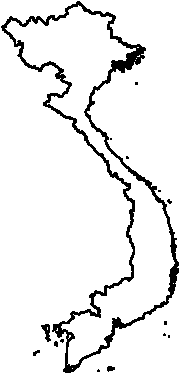
\includegraphics{geospatial_files/figure-latex/unnamed-chunk-3-1.pdf}

Notice that the \texttt{getData()} function goes to the internet to pull
the shapefile. It is best to save it to object for easier reference
later.

The object is saved as a SpatialPolygonDataFrame.

\section{Shapefile Exercise}\label{shapefile-exercise}

Get the next level of detail for Vietnam and plot it to compare the two
levels.

\section{Uploading Shapefiles}\label{uploading-shapefiles}

If you have shapefiles in the Esri format, which is actually a
collection of multiple files stored together, you can read them into R
with the \texttt{readOGR()} function in the \textbf{rgdal} package.

You can download shapefiles at the GADM website,
\url{http://www.gadm.org/}. You can also download an ``R
SpatialPolygonsDataFrame'', which you can read into R using the
\texttt{readRDS()} function in the \textbf{rgdal} package.

\section{ggmap}\label{ggmap}

The \textbf{ggmap} package pulls base maps from online map servers like
Google Maps, OpenStreetMap, or Stamen Maps.

\begin{itemize}
\tightlist
\item
  \texttt{qmap()} function accepts a text location, used to search just
  like you do at the online map.
\end{itemize}

\begin{Shaded}
\begin{Highlighting}[]
\KeywordTok{qmap}\NormalTok{(}\DataTypeTok{location =} \StringTok{"Vietnam"}\NormalTok{)}
\end{Highlighting}
\end{Shaded}

\begin{figure}
\centering
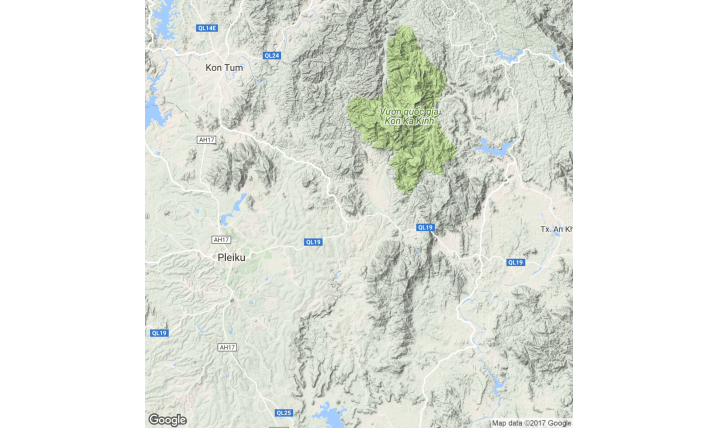
\includegraphics{qmap1.png}
\caption{}
\end{figure}

\begin{itemize}
\tightlist
\item
  ``zoom'' parameter: 3 = continent, 10 = city, 21 = building (default
  is 10, max is 21)
\end{itemize}

\begin{Shaded}
\begin{Highlighting}[]
\KeywordTok{qmap}\NormalTok{(}\DataTypeTok{location =} \StringTok{"Vietnam"}\NormalTok{, }\DataTypeTok{zoom =} \DecValTok{6}\NormalTok{)}
\end{Highlighting}
\end{Shaded}

\begin{figure}
\centering
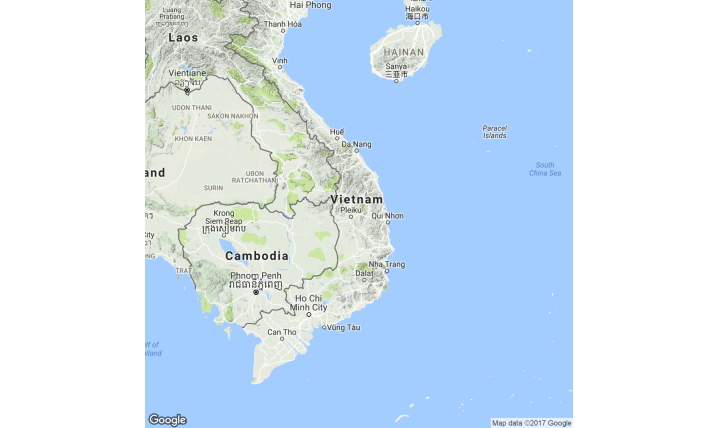
\includegraphics{qmap2.png}
\caption{}
\end{figure}

\begin{itemize}
\tightlist
\item
  ``maptype'' parameter options include terrain, satellite, roadmap, and
  hybrid.
\end{itemize}

\section{Exercise}\label{exercise}

\begin{enumerate}
\def\labelenumi{\arabic{enumi}.}
\item
  Compare the 4 map types for Fort Belvoir at zoom level 13: terrain,
  satellite, roadmap, and hybrid.
\item
  Use the coordinates for Fort Belvoir, VA in the location parameter:
  38.714668, -77.143600
\end{enumerate}

\section{Map Distance}\label{map-distance}

Calculate distance:

\begin{Shaded}
\begin{Highlighting}[]
\KeywordTok{mapdist}\NormalTok{(}\StringTok{"Washington DC"}\NormalTok{,}\StringTok{"Fort Belvoir, VA"}\NormalTok{, }\StringTok{"driving"}\NormalTok{)}
\end{Highlighting}
\end{Shaded}

\section{Geocoding}\label{geocoding}

You may have location data that does not include latitudes and
longitudes. But plotting those points requires the lat/longs. the
\texttt{geocode()} function in \textbf{ggmaps} uses Google Maps to get
the lat/longs for text locations, just like as if you were searching in
a web browser.

\begin{Shaded}
\begin{Highlighting}[]
\KeywordTok{geocode}\NormalTok{(}\StringTok{"Fort Belvoir, VA"}\NormalTok{)}
\end{Highlighting}
\end{Shaded}

\begin{verbatim}
##   lon lat
## 1  NA  NA
\end{verbatim}

\begin{Shaded}
\begin{Highlighting}[]
\KeywordTok{geocode}\NormalTok{(}\StringTok{"6001 Goethals Rd, Fort Belvoir, VA"}\NormalTok{)}
\end{Highlighting}
\end{Shaded}

\begin{verbatim}
##         lon      lat
## 1 -77.14357 38.71472
\end{verbatim}

Try geocoding with just a place name, such as ``Disney World''.

\section{Takeoff Data}\label{takeoff-data}

Using the \texttt{geocode()} function, we created a dataset with the
coordinates of the takeoff locations (not including the ships).

\begin{Shaded}
\begin{Highlighting}[]
\NormalTok{takeoff <-}\StringTok{ }\KeywordTok{read.csv}\NormalTok{(}\StringTok{"takeoff.csv"}\NormalTok{, }\DataTypeTok{stringsAsFactors =} \OtherTok{FALSE}\NormalTok{)}
\KeywordTok{head}\NormalTok{(takeoff)}
\end{Highlighting}
\end{Shaded}

\begin{verbatim}
##        takeoff      lon      lat
## 1        KORAT 102.0978 14.97990
## 2     BIEN HOA 106.8427 10.95741
## 3      CHU LAI 108.7038 15.41441
## 4 TAN SON NHUT 106.6588 10.81846
## 5       TAKHLI 100.3273 15.28435
## 6 CAM RANH BAY 109.1702 11.89333
\end{verbatim}

\chapter{Map Layers}\label{map-layers}

Now that we have basemaps, the next step is to add data to the map.

First, let's create an object that is our basemap.

\begin{Shaded}
\begin{Highlighting}[]
\NormalTok{vnmap <-}\StringTok{ }\KeywordTok{qmap}\NormalTok{(}\DataTypeTok{location =}\StringTok{"Vietnam"}\NormalTok{, }\DataTypeTok{zoom =} \DecValTok{6}\NormalTok{)}
\end{Highlighting}
\end{Shaded}

\section{Points}\label{points}

Adding data to the basemap with the \textbf{ggmap} package uses layers,
similar to \textbf{ggplot2}.

Let's add points for the takeoff locations to the basemap. Note that
``x'' should always be mapped to the variable for longitude and ``y''
mapped to latitude.

\begin{Shaded}
\begin{Highlighting}[]
\NormalTok{vnmap }\OperatorTok{+}\StringTok{ }
\StringTok{  }\KeywordTok{geom_point}\NormalTok{(}\DataTypeTok{data =}\NormalTok{ takeoff, }\KeywordTok{aes}\NormalTok{(}\DataTypeTok{x =}\NormalTok{ lon, }\DataTypeTok{y =}\NormalTok{ lat))}
\end{Highlighting}
\end{Shaded}

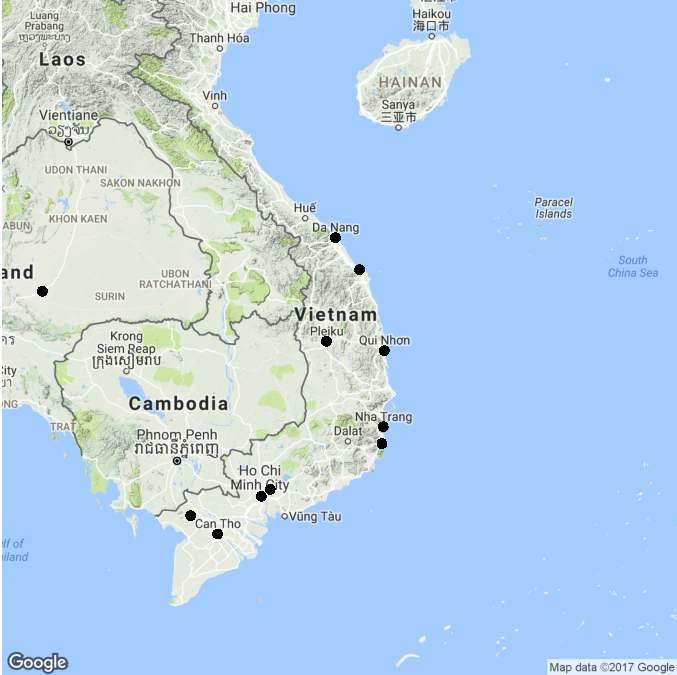
\includegraphics{geospatial_files/figure-latex/unnamed-chunk-10-1.pdf}

Format the points the same way as in \textbf{ggplot2}.

\begin{Shaded}
\begin{Highlighting}[]
\NormalTok{vnmap }\OperatorTok{+}
\StringTok{  }\KeywordTok{geom_point}\NormalTok{(}\DataTypeTok{data =}\NormalTok{ takeoff, }\KeywordTok{aes}\NormalTok{(}\DataTypeTok{x =}\NormalTok{ lon, }\DataTypeTok{y =}\NormalTok{ lat), }\DataTypeTok{shape =} \DecValTok{15}\NormalTok{, }\DataTypeTok{size =} \DecValTok{2}\NormalTok{, }\DataTypeTok{colour =} \StringTok{"purple"}\NormalTok{) }
\end{Highlighting}
\end{Shaded}

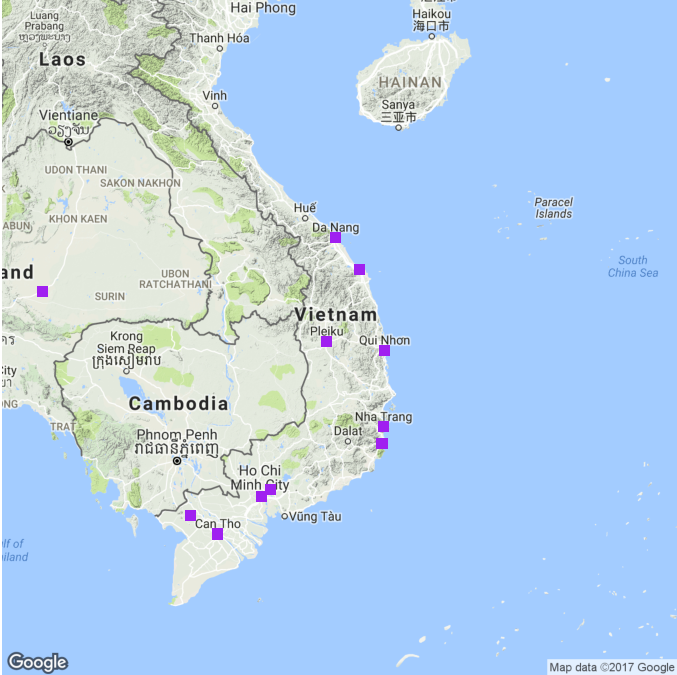
\includegraphics{geospatial_files/figure-latex/unnamed-chunk-11-1.pdf}

\section{Plot Points Exercise}\label{plot-points-exercise}

\begin{enumerate}
\def\labelenumi{\arabic{enumi}.}
\item
  Subset the ``nam65'' data set for strike missions. (Hint: variable
  MFUNC\_DESC)
\item
  Plot the strike points on the basemap.
\item
  Color the strike points based on the ``MILSERVICE'' variable.
\end{enumerate}

\section{Heat Maps}\label{heat-maps}

A heat map reflects the concentration of points on the map, also thought
of as data density.

\begin{itemize}
\item
  Use the \texttt{stat\_density2d()} function to create the heat map
  layer.
\item
  \texttt{fill} mapping provides color, \texttt{alpha} mapping adjusts
  the transparency.
\item
  Remove the legend because it doesn't provide useful information:
  \texttt{show.legend\ =\ FALSE}
\end{itemize}

\begin{Shaded}
\begin{Highlighting}[]
\NormalTok{strike <-}\StringTok{ }\NormalTok{dplyr}\OperatorTok{::}\KeywordTok{filter}\NormalTok{(nam65, MFUNC_DESC}\OperatorTok{==}\StringTok{"STRIKE"}\NormalTok{)}

\NormalTok{vnmap }\OperatorTok{+}\StringTok{ }
\StringTok{  }\KeywordTok{stat_density2d}\NormalTok{(}\DataTypeTok{data =}\NormalTok{ strike, }\KeywordTok{aes}\NormalTok{(}\DataTypeTok{x =}\NormalTok{ TGTLONDDD_DDD_WGS84, }\DataTypeTok{y =}\NormalTok{ TGTLATDD_DDD_WGS84, }
                                    \DataTypeTok{fill =}\NormalTok{ ..level.., }\DataTypeTok{alpha =}\NormalTok{ ..level..), }
                 \DataTypeTok{geom =} \StringTok{"polygon"}\NormalTok{, }\DataTypeTok{show.legend =} \OtherTok{FALSE}\NormalTok{)}
\end{Highlighting}
\end{Shaded}

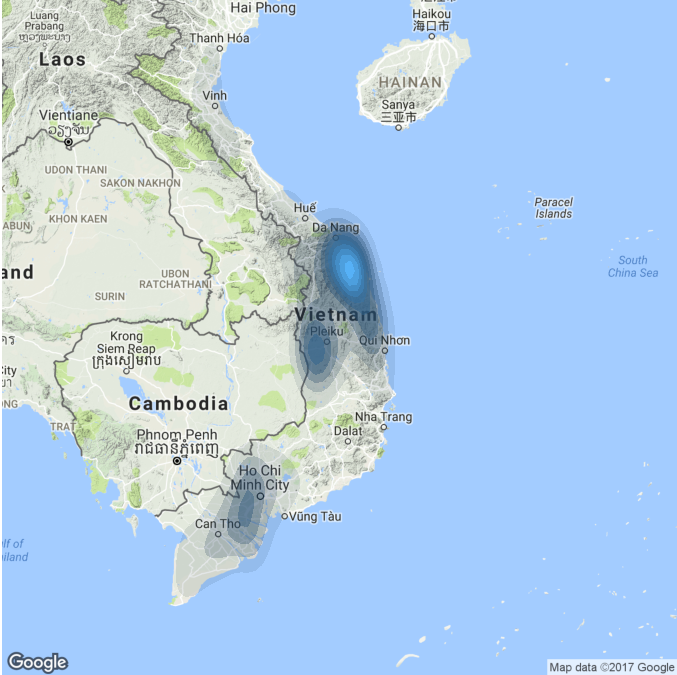
\includegraphics{geospatial_files/figure-latex/unnamed-chunk-12-1.pdf}

\section{Facet the Maps}\label{facet-the-maps}

You can facet maps just like plots!

\begin{itemize}
\tightlist
\item
  Use \texttt{facet\_wrap()} to organize the sub-maps with the same
  number of rows and columns.
\end{itemize}

\begin{Shaded}
\begin{Highlighting}[]
\NormalTok{vnmap }\OperatorTok{+}
\StringTok{  }\KeywordTok{stat_density2d}\NormalTok{(}\DataTypeTok{data =}\NormalTok{ strike, }\KeywordTok{aes}\NormalTok{(}\DataTypeTok{x =}\NormalTok{ TGTLONDDD_DDD_WGS84, }\DataTypeTok{y =}\NormalTok{ TGTLATDD_DDD_WGS84,}
                                    \DataTypeTok{fill =}\NormalTok{ ..level.., }\DataTypeTok{alpha =}\NormalTok{ ..level..),}
                 \DataTypeTok{geom =} \StringTok{"polygon"}\NormalTok{, }\DataTypeTok{show.legend =} \OtherTok{FALSE}\NormalTok{) }\OperatorTok{+}
\StringTok{  }\KeywordTok{facet_wrap}\NormalTok{(}\OperatorTok{~}\StringTok{ }\NormalTok{MILSERVICE)}
\end{Highlighting}
\end{Shaded}

\begin{verbatim}
## Warning: Removed 1378 rows containing non-finite values (stat_density2d).
\end{verbatim}

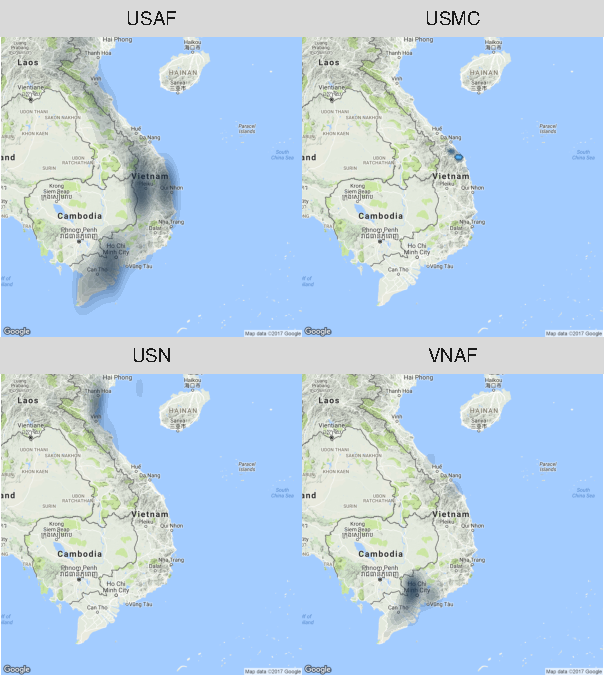
\includegraphics{geospatial_files/figure-latex/unnamed-chunk-13-1.pdf}

\chapter{Leaflet}\label{leaflet}

Leaflet is a library for making interactive maps. The JavaScript version
of leaflet is used by many websites and GIS specialists.

Here's a tutorial for leaflet: \url{http://rstudio.github.io/leaflet/}

\section{Leaflet Basemaps}\label{leaflet-basemaps}

Just like \textbf{ggplot2}, leaflet creates visualization in layers.

\begin{enumerate}
\def\labelenumi{\arabic{enumi}.}
\item
  Start with \texttt{leaflet()} to create a map widget.
\item
  Add a map tiles layer. The default layer is an OpenStreetMap map, with
  \texttt{addTiles()}.
\item
  Use \texttt{setView()} to center the map and set the zoom level.
\item
  Separate layers with a pipe operator \texttt{\%\textgreater{}\%}, not
  the plus sign.
\end{enumerate}

\begin{Shaded}
\begin{Highlighting}[]
\KeywordTok{leaflet}\NormalTok{() }\OperatorTok
\StringTok{  }\KeywordTok{addTiles}\NormalTok{() }\OperatorTok
\StringTok{  }\KeywordTok{setView}\NormalTok{(}\DataTypeTok{lng =} \DecValTok{107}\NormalTok{, }\DataTypeTok{lat =} \DecValTok{17}\NormalTok{, }\DataTypeTok{zoom =} \DecValTok{6}\NormalTok{)}
\end{Highlighting}
\end{Shaded}

Notice that OpenStreetMap uses the local language on the map, which is
not useful for our purposes.

The \texttt{addProviderTiles()} function sets the basemap you want to
use, which are also called ``providers''. The list of providers that you
can reference with leaflet can be found
\href{https://leaflet-extras.github.io/leaflet-providers/preview/}{here}
and in this case we chose ``Esri.WorldTopoMap''.

\begin{Shaded}
\begin{Highlighting}[]
\KeywordTok{leaflet}\NormalTok{() }\OperatorTok
\StringTok{  }\KeywordTok{setView}\NormalTok{(}\DataTypeTok{lng =} \DecValTok{107}\NormalTok{, }\DataTypeTok{lat =} \DecValTok{17}\NormalTok{, }\DataTypeTok{zoom =} \DecValTok{6}\NormalTok{) }\OperatorTok
\StringTok{  }\KeywordTok{addProviderTiles}\NormalTok{(}\StringTok{"Esri.WorldTopoMap"}\NormalTok{)}
\end{Highlighting}
\end{Shaded}

\section{Add Points}\label{add-points}

Using the strike dataframe, we will add markers on the map for the
locations of the strike missions.

\begin{itemize}
\item
  Strike data:
  \texttt{strike\ \textless{}-\ dplyr::filter(nam65,\ MFUNC\_DESC=="STRIKE")}
\item
  Use \texttt{addCircleMarkers()} to add points to the base map.
\item
  Be sure to add the tilde (\textasciitilde{}) before the variable
  names.
\item
  Note: Leaflet stops plotting points after it hits an NA in the
  latitude or longitude variable, so be sure to filter out any rows with
  NAs in the geospatial variables.
\end{itemize}

\begin{Shaded}
\begin{Highlighting}[]
\KeywordTok{leaflet}\NormalTok{() }\OperatorTok
\StringTok{  }\KeywordTok{setView}\NormalTok{(}\DataTypeTok{lng =} \DecValTok{107}\NormalTok{, }\DataTypeTok{lat =} \DecValTok{17}\NormalTok{, }\DataTypeTok{zoom =} \DecValTok{6}\NormalTok{) }\OperatorTok
\StringTok{  }\KeywordTok{addProviderTiles}\NormalTok{(}\StringTok{"Esri.WorldTopoMap"}\NormalTok{) }\OperatorTok
\StringTok{  }\KeywordTok{addCircleMarkers}\NormalTok{(}\DataTypeTok{data =}\NormalTok{ strike, }\DataTypeTok{lng=}\OperatorTok{~}\NormalTok{TGTLONDDD_DDD_WGS84, }\DataTypeTok{lat=}\OperatorTok{~}\NormalTok{TGTLATDD_DDD_WGS84, }
                   \DataTypeTok{radius =} \DecValTok{2}\NormalTok{)}
\end{Highlighting}
\end{Shaded}

\section{Add Popups}\label{add-popups}

A great feature of interactive maps is popups that provide information
when the user clicks on the marker.

\begin{itemize}
\item
  Use the ``popup'' parameter in the \texttt{addCircleMarker()} layer.
\item
  We want the popup to show the service that flew the mission.
\end{itemize}

\begin{Shaded}
\begin{Highlighting}[]
\KeywordTok{leaflet}\NormalTok{() }\OperatorTok
\StringTok{  }\KeywordTok{setView}\NormalTok{(}\DataTypeTok{lng =} \DecValTok{107}\NormalTok{, }\DataTypeTok{lat =} \DecValTok{17}\NormalTok{, }\DataTypeTok{zoom =} \DecValTok{6}\NormalTok{) }\OperatorTok
\StringTok{  }\KeywordTok{addProviderTiles}\NormalTok{(}\StringTok{"Esri.WorldTopoMap"}\NormalTok{) }\OperatorTok
\StringTok{  }\KeywordTok{addCircleMarkers}\NormalTok{(}\DataTypeTok{data =}\NormalTok{ strike, }\DataTypeTok{lng =} \OperatorTok{~}\NormalTok{TGTLONDDD_DDD_WGS84, }\DataTypeTok{lat =} \OperatorTok{~}\NormalTok{TGTLATDD_DDD_WGS84, }
                   \DataTypeTok{radius =} \DecValTok{2}\NormalTok{, }\DataTypeTok{popup =} \OperatorTok{~}\NormalTok{strike}\OperatorTok{$}\NormalTok{MILSERVICE)}
\end{Highlighting}
\end{Shaded}

You can add multiple fields to the popup by combining them with the
\texttt{paste()} function like:

\texttt{popup\ =\ paste("Service:",\ strike\$MILSERVICE,",\ ",strike\$TAKEOFFLOCATION)}

\section{Saving Maps}\label{saving-maps}

You can save maps to use outside RStudio, ust like other visualizations,
by clicking the ``Export'' dropdown on the ``Plots'' tab.

Options: 1. Save as Image. 2. Save as PDF. 3. Copy to Clipboard.

To save a leaflet map:

\begin{itemize}
\item
  Click the ``Export'' dropdown on the ``Viewer'' tab.
\item
  Click ``Save as a Webpage''. This will create an html file for the
  leaflet map.
\item
  Name the html file. It will default to saving in your working
  directory.
\end{itemize}

\section{Leaflet Exercise}\label{leaflet-exercise}

\begin{enumerate}
\def\labelenumi{\arabic{enumi}.}
\item
  Plot the locations of strike missions by the B-57 aircraft on an Esri
  World Street Map basemap.
\item
  Popup the target type and operation supported.
\end{enumerate}

\section{Colors and Legends}\label{colors-and-legends}

\begin{itemize}
\item
  To color the points based on another variable, you need to define a
  palette for that variable and then reference it in the \texttt{color}
  parameter in \texttt{addCircleMarkers}.
\item
  Use the \texttt{addLegend()} function to add a legend for those
  colors, again referencing the defined palette.
\end{itemize}

\begin{Shaded}
\begin{Highlighting}[]
\NormalTok{svc_pal <-}\StringTok{ }\KeywordTok{colorFactor}\NormalTok{(}\KeywordTok{c}\NormalTok{(}\StringTok{"blue"}\NormalTok{,}\StringTok{"red"}\NormalTok{,}\StringTok{"orange"}\NormalTok{,}\StringTok{"green"}\NormalTok{), strike}\OperatorTok{$}\NormalTok{MILSERVICE)}

\KeywordTok{leaflet}\NormalTok{() }\OperatorTok
\StringTok{  }\KeywordTok{setView}\NormalTok{(}\DataTypeTok{lng =} \DecValTok{107}\NormalTok{, }\DataTypeTok{lat =} \DecValTok{17}\NormalTok{, }\DataTypeTok{zoom =} \DecValTok{6}\NormalTok{) }\OperatorTok
\StringTok{  }\KeywordTok{addProviderTiles}\NormalTok{(}\StringTok{"Esri.WorldTopoMap"}\NormalTok{) }\OperatorTok
\StringTok{  }\KeywordTok{addCircleMarkers}\NormalTok{(}\DataTypeTok{data =}\NormalTok{ strike, }\DataTypeTok{lng =} \OperatorTok{~}\NormalTok{TGTLONDDD_DDD_WGS84, }\DataTypeTok{lat =} \OperatorTok{~}\NormalTok{TGTLATDD_DDD_WGS84, }
                   \DataTypeTok{radius =} \DecValTok{2}\NormalTok{, }\DataTypeTok{popup =} \OperatorTok{~}\NormalTok{strike}\OperatorTok{$}\NormalTok{MILSERVICE,}
                   \DataTypeTok{color =} \OperatorTok{~}\KeywordTok{svc_pal}\NormalTok{(MILSERVICE)) }\OperatorTok
\StringTok{  }\KeywordTok{addLegend}\NormalTok{(}\DataTypeTok{pal =}\NormalTok{ svc_pal, }\DataTypeTok{values =}\NormalTok{ strike}\OperatorTok{$}\NormalTok{MILSERVICE)}
\end{Highlighting}
\end{Shaded}

\section{Polygon Layer}\label{polygon-layer}

Add a polygon layer with the \texttt{addPolygons()} function.

We will add the provinces of Vietnam to our map using the ``vt1''
shapefile object we created earlier.

\begin{Shaded}
\begin{Highlighting}[]
\NormalTok{vt1 <-}\StringTok{ }\KeywordTok{getData}\NormalTok{(}\StringTok{'GADM'}\NormalTok{, }\DataTypeTok{country =} \StringTok{'Vietnam'}\NormalTok{, }\DataTypeTok{level =} \DecValTok{1}\NormalTok{)}

\KeywordTok{leaflet}\NormalTok{() }\OperatorTok
\StringTok{  }\KeywordTok{setView}\NormalTok{(}\DataTypeTok{lng =} \DecValTok{107}\NormalTok{, }\DataTypeTok{lat =} \DecValTok{17}\NormalTok{, }\DataTypeTok{zoom =} \DecValTok{6}\NormalTok{) }\OperatorTok
\StringTok{  }\KeywordTok{addProviderTiles}\NormalTok{(}\StringTok{"Esri.WorldTopoMap"}\NormalTok{) }\OperatorTok
\StringTok{  }\KeywordTok{addPolygons}\NormalTok{(}\DataTypeTok{data =}\NormalTok{ vt1, }\DataTypeTok{fillOpacity =}\NormalTok{ .}\DecValTok{1}\NormalTok{, }\DataTypeTok{color =} \StringTok{"purple"}\NormalTok{)}
\end{Highlighting}
\end{Shaded}

\section{Layer Control}\label{layer-control}

If you have multiple layers on a map, you can add the functionality to
turn them on and off with the \texttt{addLayersControl()} function. You
must identify each layer you want to control with a \texttt{group}
parameter in the layer information.

We will add the circle markers back onto the map along with the layers
control.

\begin{Shaded}
\begin{Highlighting}[]
\KeywordTok{leaflet}\NormalTok{() }\OperatorTok
\StringTok{  }\KeywordTok{setView}\NormalTok{(}\DataTypeTok{lng =} \DecValTok{107}\NormalTok{, }\DataTypeTok{lat =} \DecValTok{17}\NormalTok{, }\DataTypeTok{zoom =} \DecValTok{6}\NormalTok{) }\OperatorTok
\StringTok{  }\KeywordTok{addProviderTiles}\NormalTok{(}\StringTok{"Esri.WorldTopoMap"}\NormalTok{) }\OperatorTok
\StringTok{  }\KeywordTok{addCircleMarkers}\NormalTok{(}\DataTypeTok{data =}\NormalTok{ strike, }\DataTypeTok{lng =} \OperatorTok{~}\NormalTok{TGTLONDDD_DDD_WGS84, }\DataTypeTok{lat =} \OperatorTok{~}\NormalTok{TGTLATDD_DDD_WGS84, }
                   \DataTypeTok{radius =} \DecValTok{2}\NormalTok{, }\DataTypeTok{popup =} \OperatorTok{~}\NormalTok{strike}\OperatorTok{$}\NormalTok{MILSERVICE, }\DataTypeTok{group =} \StringTok{"Strike"}\NormalTok{) }\OperatorTok
\StringTok{  }\KeywordTok{addPolygons}\NormalTok{(}\DataTypeTok{data =}\NormalTok{ vt1, }\DataTypeTok{fillOpacity =}\NormalTok{ .}\DecValTok{1}\NormalTok{, }\DataTypeTok{color =} \StringTok{"purple"}\NormalTok{, }\DataTypeTok{group =} \StringTok{"Province"}\NormalTok{) }\OperatorTok
\StringTok{  }\KeywordTok{addLayersControl}\NormalTok{(}\DataTypeTok{overlayGroups =} \KeywordTok{c}\NormalTok{(}\StringTok{"Strike"}\NormalTok{,}\StringTok{"Province"}\NormalTok{))}
\end{Highlighting}
\end{Shaded}

\section{Leaflet Strikes Exercise}\label{leaflet-strikes-exercise}

\begin{enumerate}
\def\labelenumi{\arabic{enumi}.}
\item
  Create a map of strikes with layer control and different colors for
  each military service.
\item
  Hint: subset by service.
\end{enumerate}


\end{document}
